\section{Figures for brute force metropolis and importance sampling}
\begin{figure}[h]
\hspace{-2.8cm}
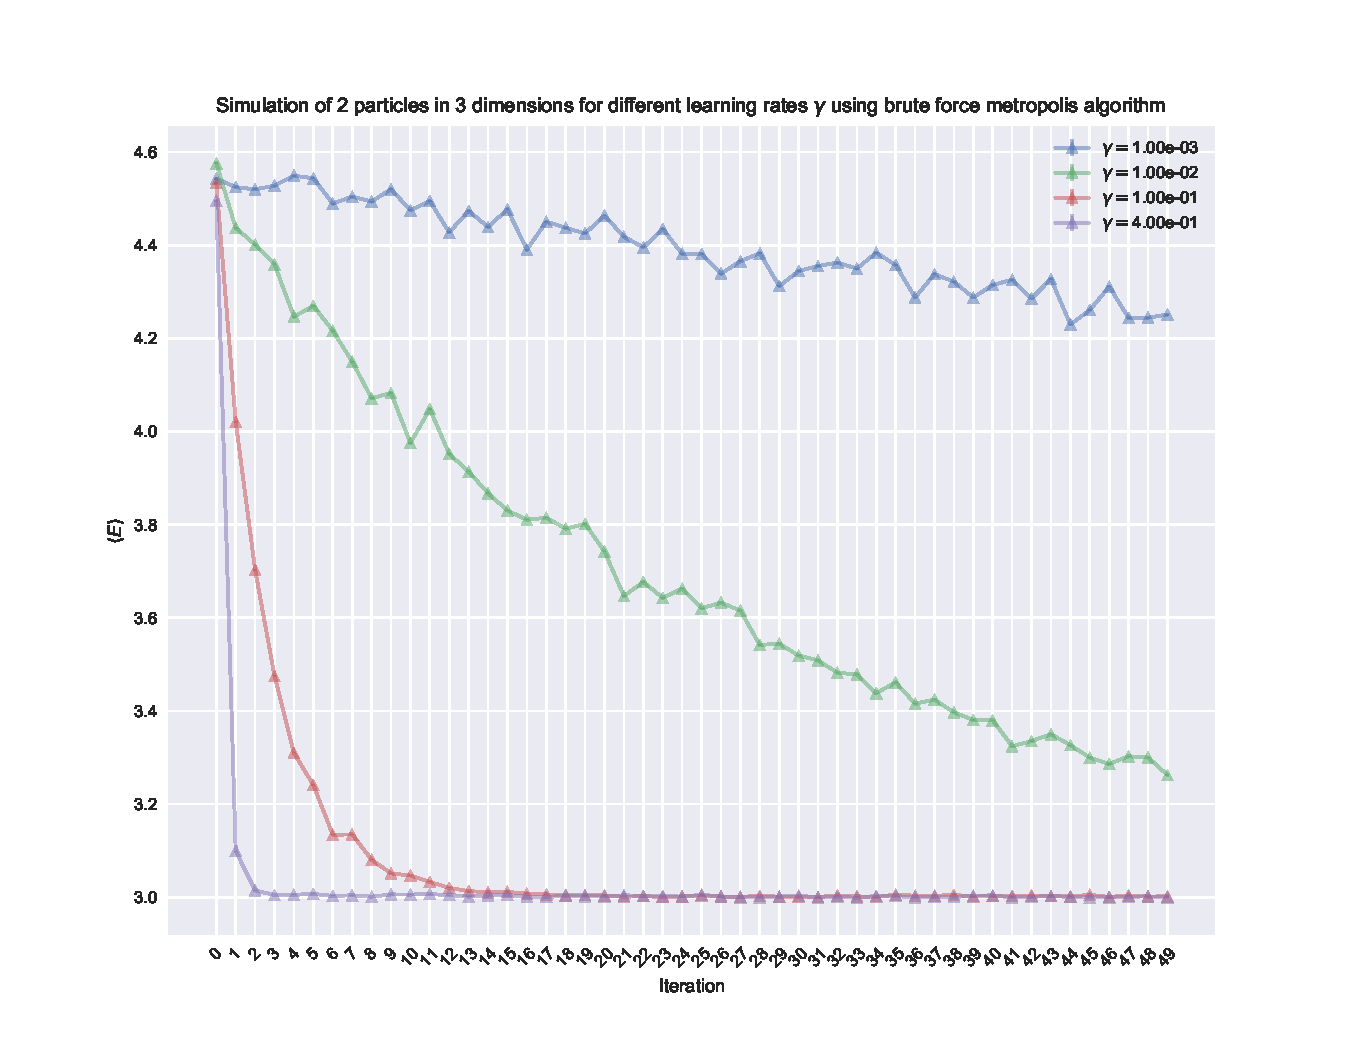
\includegraphics[width = \paperwidth]{figures/naive_2p_3d.pdf}
\caption{Plot of simulation with 2 particles in 3 dimensions with varied learning rates $\gamma$, using brute force metropolis sampling.
			2 hidden nodes were used.
			For detailed values on energy, variance, and CPU-time per mc-cycle, see table \ref{tab:naive-nin}}
\label{fig:naive-nin}
\end{figure}


\begin{figure}[h]
\hspace{-2.8cm}
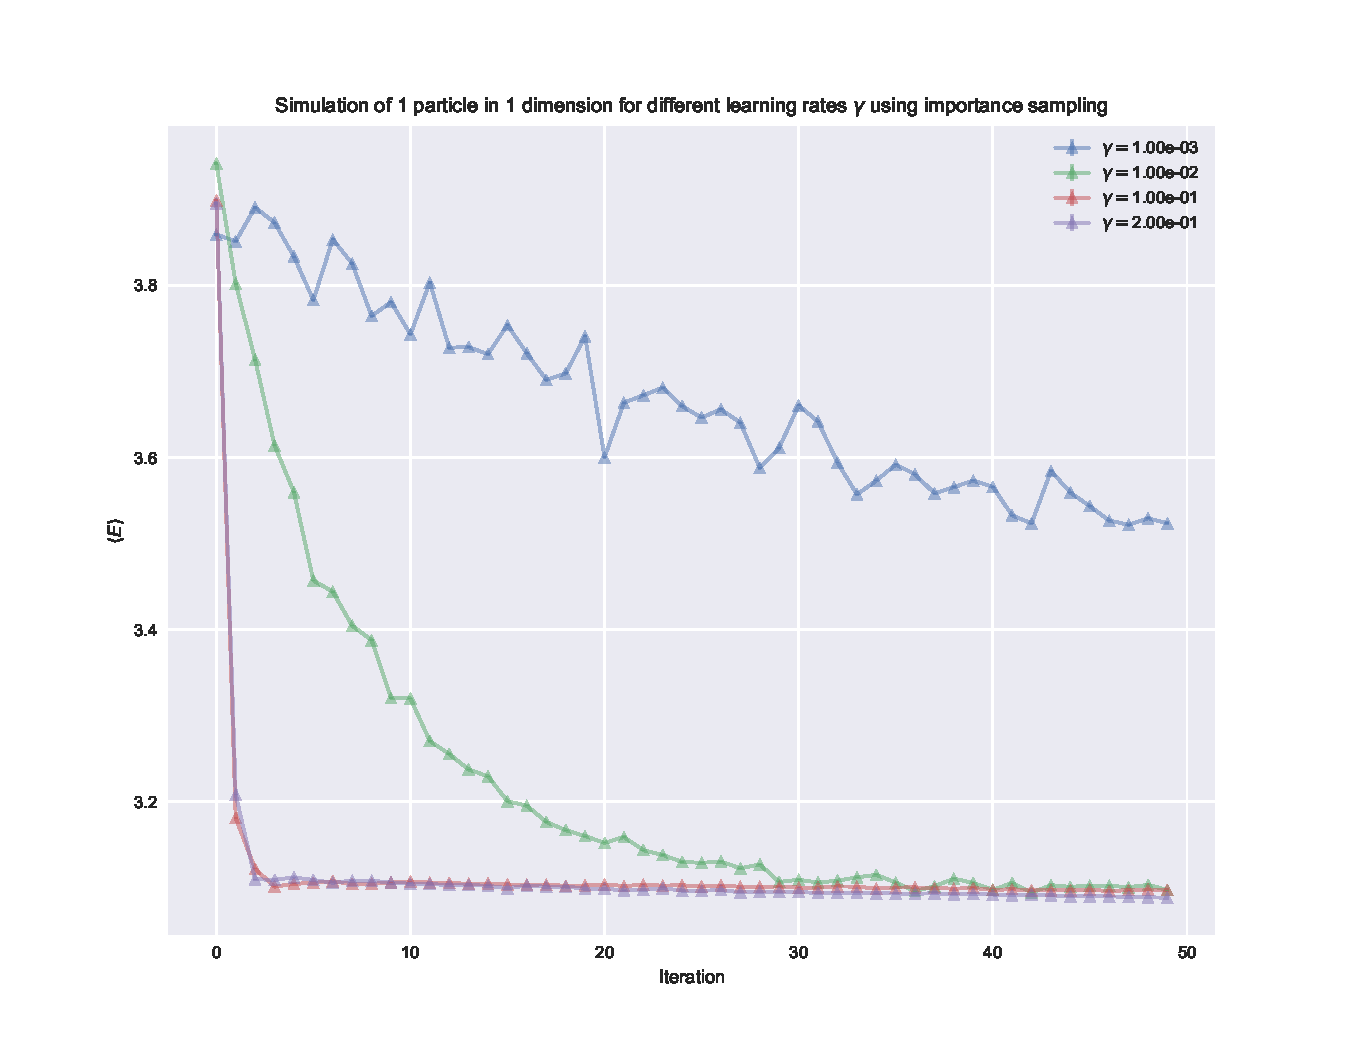
\includegraphics[width = \paperwidth]{figures/importance_2p_3d.pdf}
\caption{Plot of simulation with 2 particles in 3 dimensions with varied learning rates $\gamma$, using brute force metropolis sampling.
			For detailed values on energy, variance, and CPU-time per mc-cycle, see table \ref{tab:importance-nin-gamma}}
\label{fig:importance-nin-gamma}
\end{figure}


\begin{figure}[h]
\hspace{-2.8cm}
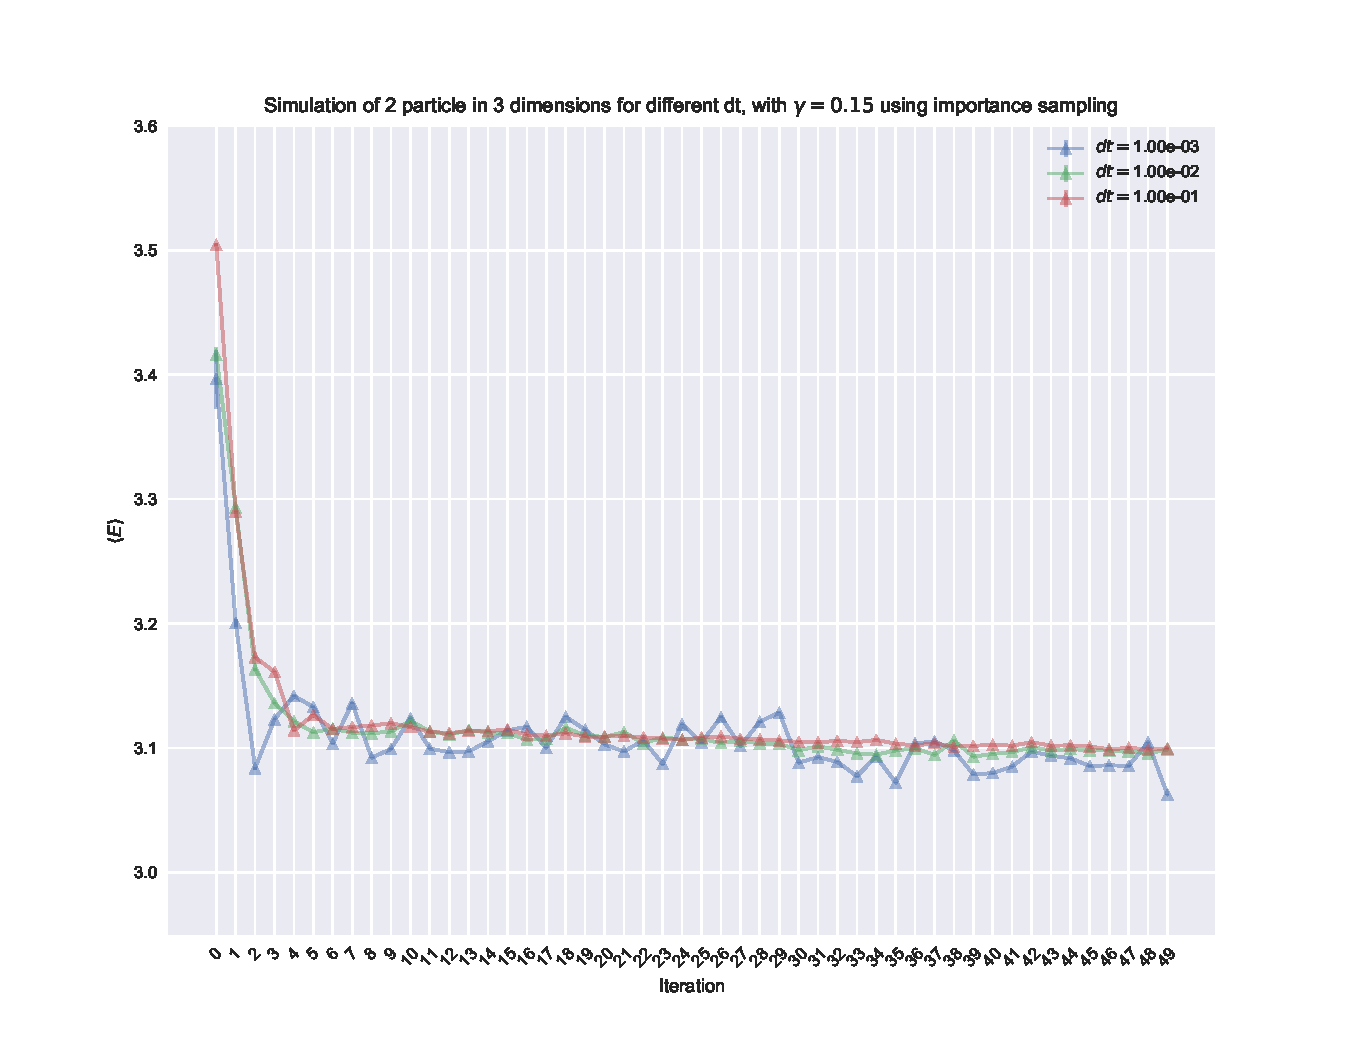
\includegraphics[width = \paperwidth]{figures/importance_2p_3d_dt.pdf}
\caption{Plot of simulation with 2 particles in 3 dimensions with varied learning rates $\gamma$, using brute force metropolis sampling.
			For detailed values on energy, variance, and CPU-time per mc-cycle, see table \ref{tab:importance-nin-dt}}
\label{fig:importance-nin-dt}
\end{figure}
